\documentclass[12pt,letterpaper]{hmcpset}
\usepackage[margin=1in]{geometry} 
\usepackage{graphicx}
\usepackage{amsmath}
\usepackage{url}

% info for header block in upper right hand corner
\name{}
\class{Math 45 - Section --- \hspace{20pt}}
\assignment{HW 11}
\duedate{Tuesday, April 26, 2016}

\newcommand{\pn}[1]{\left( #1 \right)}
\newcommand{\abs}[1]{\left| #1 \right|}
\newcommand{\bk}[1]{\left[ #1 \right]}

% Start enumerates at a) instead of 1
\renewcommand{\labelenumi}{{(\alph{enumi})}}

%Block Paragraphs
\setlength{\parindent}{0pt}
\setlength{\parskip}{1em}

\begin{document}

\problemlist{1, 2}

\begin{problem}[1]
    The forced motion of a mass suspended from the ceiling with a
    spring obeys the equation
    $$m y''(t)+ c y'(t)+k y(t) = F_0 \sin(\omega t).$$
    Use the constants $m=1$, $c=4$, $k=5$, $F_0=1$ and
    $\omega=4$. Suppose that initially the mass is released from the
    position $y=2$ with no velocity, that is, $y(0)=2$ and $y'(0)=0$.
    \begin{enumerate}
        \item Solve for $y(t)$ using the method of undetermined coefficients.
        \item Identify those terms in your solution $y(t)$ that correspond to
            the transient behavior of the system, and those that correspond to
            the forced response of the system.
    \end{enumerate}
\end{problem}

%p1%
\begin{solution}
    \vfill
\end{solution}
\newpage

\begin{problem}[2]
    A $m$~kg mass is suspended at the end of a (massless) rod with length $L$~meters. The other end of the rod is fixed at a pivot point. This arrangement that leads to a simple pendulum that swings in a plane.
    \begin{center}
        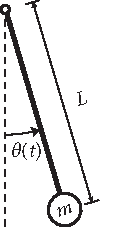
\includegraphics[width=.75in,keepaspectratio=true]{img/apr_26_2_pendulum.pdf}
    \end{center}

    \vspace{-.2in}Suppose that there is no air resistance, friction, or any other mechanism that causes the pendulum to lose energy. The only force acting on the pendulum is the force of gravity pulling the mass down.  Let $\theta(t)$ be the angular position of the pendulum, measured so that the resting position of the pendulum corresponds to $\theta=0$ and positive $\theta$ is in the direction of the arrow above. In this problem, you will derive the governing equation of the pendulum's motion in two different ways.
    \begin{enumerate}
        \item First, you will derive a governing equation using the rotational analog of Newton's second law, $\tau=I\ddot{\theta}$.  (See Chapter 18 of your Physics 24 textbook.) You can assume that the mass is concentrated at a point and the rod is massless, so the moment of inertia of the mass is $I=mL^2$.  Calculate the torque that results from the force of gravity acting on the mass to obtain a differential equation for $\theta(t)$.
        \item Now, you will rederive the same equation using conservation of energy.  (See Chapter 19 of your Physics 24 textbook.)  The total energy of the pendulum is a sum of its potential and kinetic energy.  Its kinetic energy is $\tfrac{1}{2}I\omega^2$, where $\omega=\dot{\theta}$ is the angular velocity of the mass about the pivot point.  Calculate the potential energy of the mass, relative to the lowest point that the mass can attain (at $\theta=0$).  Write down an expression for the total energy $E(t)$ of the pendulum, then take a derivative of the $E(t)$, remembering to use the chain rule properly. Use the fact that the derivative of $E(t)$ should be zero, since the total energy of the pendulum is constant, to derive a differential equation for $\theta(t)$.  After some algebraic simplification, you should arrive at the same differential equation as in part (a).
    \end{enumerate}
\end{problem}
\newpage

%p2%
\begin{solution}
    \null\vfill
\end{solution}
\newpage

\begin{problem}[3]
    In the previous problem, you found that the DE $\ddot{\theta}+\frac{g}{L}\sin\theta=0$ describes the motion of a simple, undamped pendulum.  In this problem, we explore some numerical solutions of this DE obtained using PPLANE (\url{http://math.rice.edu/~dfield/dfpp.html}).  

    \begin{center}
        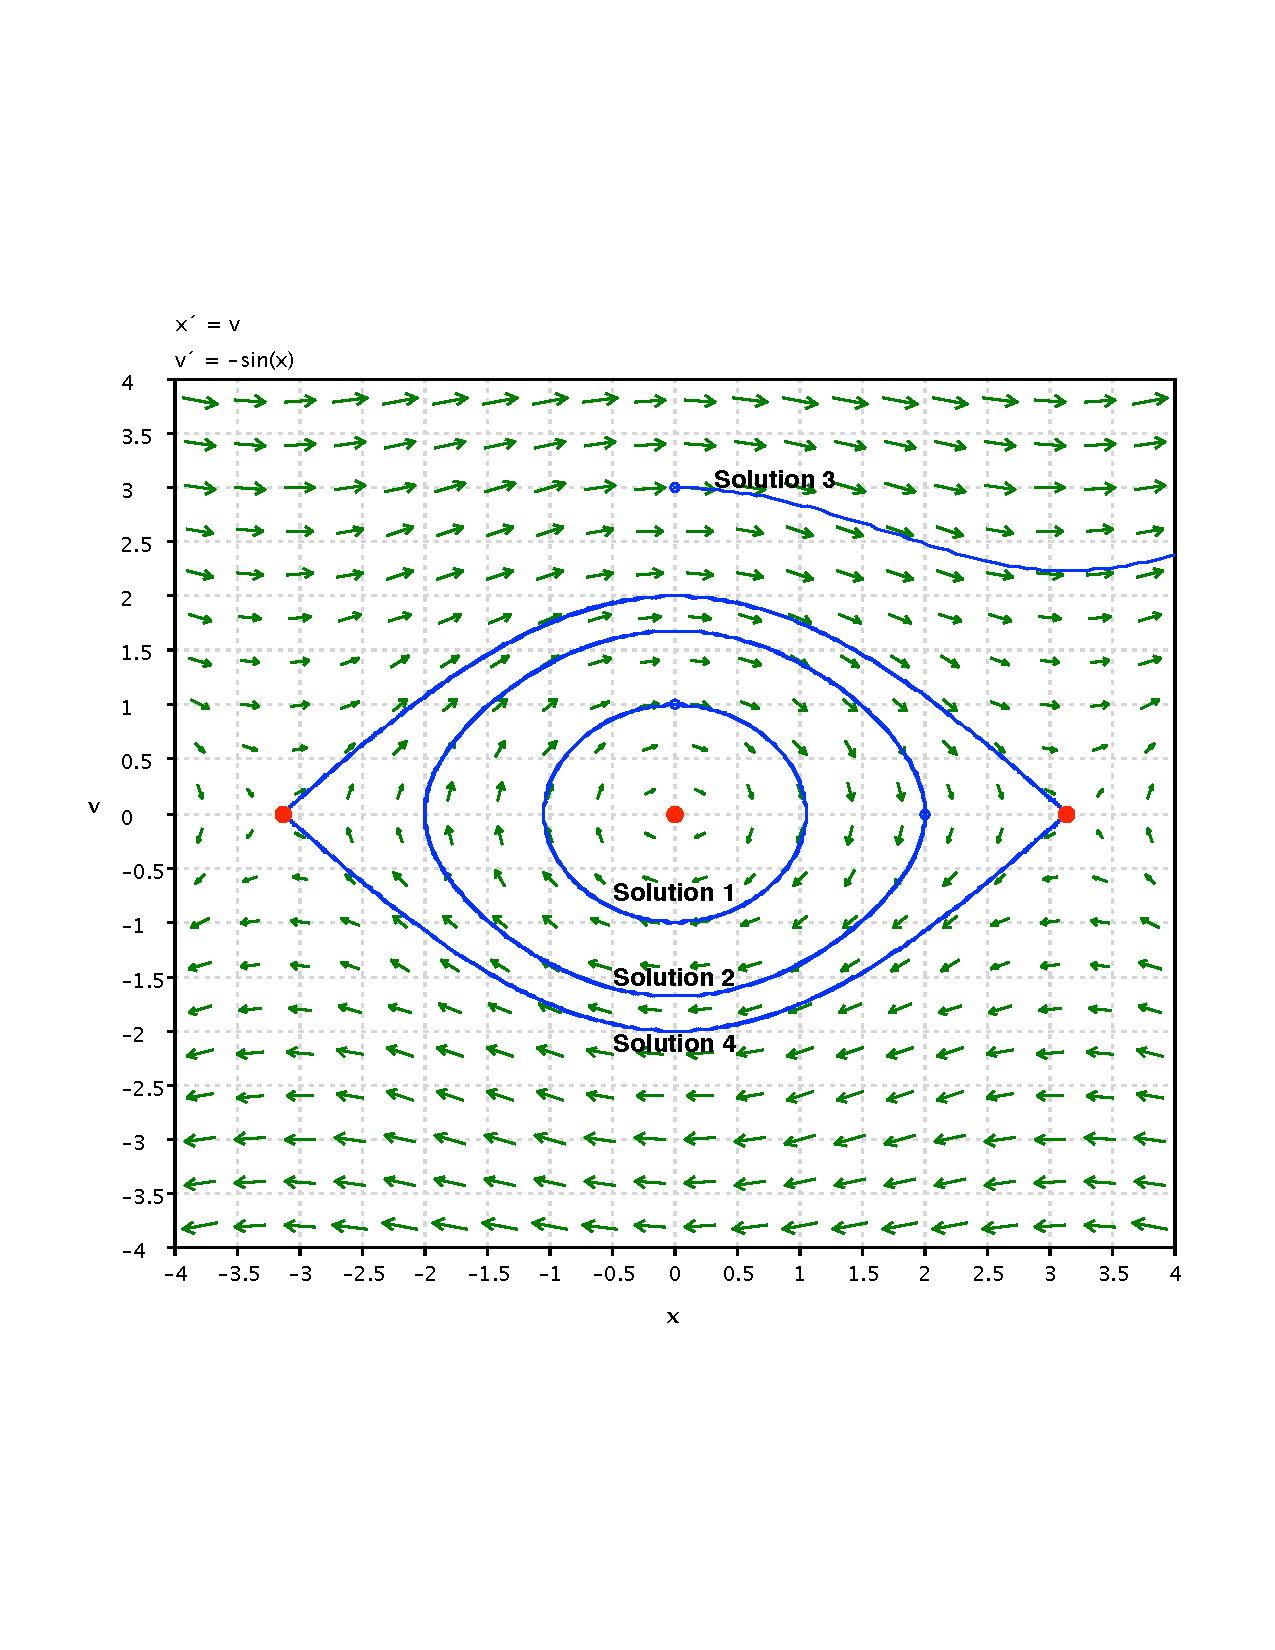
\includegraphics[width=4in,keepaspectratio=true]{img/apr_26_3_graph.pdf}
    \end{center}

    First, we need to explain a few things.  To use PPLANE, we rename $\theta=x$ and $\dot{\theta}=v$.  (The reason we need to use $x$ and $v$ is that PPLANE doesn't allow for more complicated variable names.)  We rewrite the second-order DE $\ddot{\theta}=-\frac{g}{L}\sin\theta$ as a pair of two first-order differential equations:
    \[
        x'=v \qquad \text{and} \qquad v'=-\frac{g}{L}\sin x
    \]
    The first equation comes from the fact that $x=\theta$ and $v=\dot{\theta}$.  The second equation comes from replacing $\ddot{\theta}$ with $v'$ in the differential equation.  Finally, we assume that $g=9.8\text{~m/s}^2$ and $L=9.8$~m so that the second equation becomes $v'=-\sin x$.  Armed with all of that information, now you're ready to watch this video:

    \begin{center}
        \url{http://www.screencast.com/t/8xUqAwok}
    \end{center}

    The video shows a picture of the \textit{phase plane} for this differential equation. The green arrows in the phase plane form a \textit{slope field} (a.k.a.~\textit{direction field}).  This slope field is similar to the ones we've seen before for first-order DEs in that in that solutions in the plane must have a tangent vector matching the slope field.  What's different about this phase plane is that the independent variable ($t$) is not one of the axes. The horizontal axis in the graph is $x$ (angular position of the pendulum) and the vertical axis is $v$ (angular velocity of the pendulum). Solutions in the phase plane are parametric curves $(x(t),v(t))$.  
\end{problem}

\begin{problem}[3 cont.]
    \begin{enumerate}
        \item In the video, Prof.~Thompson shows that the pendulum DE has three equilibrium solutions (points) at $x=-\pi$ and $v=0$, $x=0$ and $v=0$, and $x=\pi$ and $v=0$. Describe the corresponding configuration of the pendulum that corresponds to each of these three points, and explain why these configurations are equilibrium configurations of the pendulum.
        \item In the video, Prof.~Thompson plots a numerical solution with the initial condition $x(0)=0$~rads and $v(0)=1$~rads/s.  (This is marked as ``Solution 1'' in the figure above.) That solution corresponds to a specific motion of the pendulum. Describe that motion.
        \item Describe the motion of the pendulum corresponding to the solution with initial condition $x(0)=2$~rads and $v(0)=0$~rads/s.
        \item Describe the motion of the pendulum corresponding to the solution with initial condition $x(0)=0$~rads and $v(0)=3$~rads/s.
        \item Describe the motion of the pendulum corresponding to the solution with initial condition $x(0)=-3.141$~rads and $v(0)=0$~rads/s.
    \end{enumerate}
\end{problem}

\newpage
%p3%
\begin{solution}
    \null\vfill
\end{solution}
\end{document}
